\ofsubsection{Chaos in Cornelia}
%
\ofquote{"I, Garland will knock you all down!"\\}{Garland}\\
%
\begin{center} 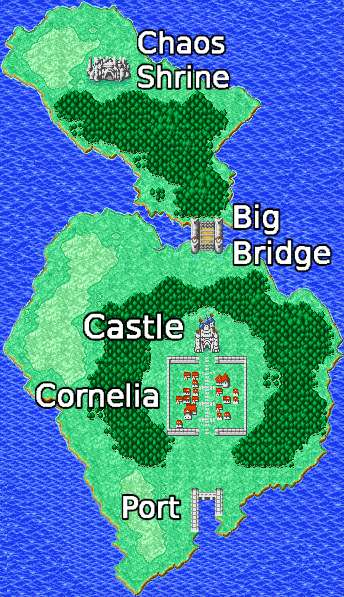
\includegraphics[width=\columnwidth]{./art/chaosincornelia/map.jpg} \end{center}
%
\accf{Chaos in Cornelia} is a pre-prepared adventure that is suitable for inexperienced players and GMs.
In this adventure, the party is tasked with finding the abducted princess Sarah of Cornelia, a plot based on the beginning of the first Final Fantasy game.
A map with all interesting locations is shown below.
The players can create their characters by following the standard character creation rules.
Since the adventure starts on a ship to Cornelia, their stories should explain why they set off on this journey.
All characters start at Level 1 with the following equipment: a Level~1 Mythril weapon they can use, Clothes, a Potion and 100 Gil.
%
\ofpar
%
\ofquote{"The moon'd tire of waitin' around for your ass!"\\}{Cid}\\\\
%
The party is on a small transport ship named \accf{Tiny Bronco}, which is on its way to deliver cargo to Cornelia.
Captain has agreed to let the party board the ship for a small fee and apart from there are only two more sailors on the ship named Biggs and Wedge.
The two sailors are wearing white bandannas and shorts as well as red shirts with stripes. 
Both of them are young and inexperienced, but friendly towards the party.
The same cannot be said of the older captain, who retreats to his cabin and prefers to be left alone.
%
\ofpar
%
\ofquote{"I don’t look like it, but I’m a coward at heart."\\}{Wedge}\\\\
%
If the adventurers are not familiar beforehand, they should introduce each other first after which they are free to explore the ship.
They can also talk to the sailors who are happy to kill time during the journey.
Biggs and Wedge tell them about recent pirate attacks on sea, which seem to have increased recently.
Furthermore, they also tell the party about Cornelia, as they have heard that the princess has disappeared.
If they ask about Cid, the sailors tell them about his past as a former soldier. 
As it starts getting dark outside, the crew retreats to their cabins.
When the adventurers prepare to finish the day, they suddenly hear loud noises surrounding the ship.
They quickly realize that several pirates have boarded the Tiny Bronco!
In the ensuing battle, the enemy party should consist of roughly one Pirate per player and due to restricted space 
you can assume that all participants within distance of each other.
Meanwhile, the crew is out of sight, fighting other pirates who have entered the ship below deck.
When the pirates are defeated, remember to award the party with the dropped Gil for each slain enemy.
%
\vfill
%
\ofmonster{Pirate}{1}{
\includegraphics[width=0.2\columnwidth]{./art/chaosincornelia/pirate.jpg}}
{
	HP: & \hfill 10 & MP: & \hfill 0\\
	STR: & \hfill 1 & DEF: & \hfill 0 \\
	MAG: & \hfill 0 & RES: & \hfill 0 \\
	AGI: & \hfill 3 & Size: & \hfill M\\
}
{\accf{Scimitar}: 1d DMG \hfill \accf{Drops:} 150 Gil}
{}
%
\vfill
%
After the battle, the crew comes together with the party and Cid thanks them for their help.
He explains that this is not the first time they have been raided by these pirates, who are part of Captain Bikke's crew.
The party may now go to sleep below deck to fully recover their HP and MP.
Shortly after they wake up in the morning, the ship arrives at Cornelia Port. 
Once there, the crew begins unloading the goods and parts ways with the party.
Cornelia Port is small and accommodates only a handful of cargo ships like the Tiny Bronco.
The sailors at the port are unloading boxes from the ships, either to store them in warehouses or carry them directly to Cornelia.
%
\\\\
%
\ofquote{"By the by, you need anything? Take a look at my wares! You might just be surprised at what you find..."}{Dyce}
%
\clearpage
%
After getting off the ship, the party can ask around to find the way to Cornelia.
The sailors warn them to be careful on the way, as the castle guards are not patrolling the route anymore.
Cornelia is not far from the port and the path mostly leads through fields and grassland.
The party can meet a traveling merchant named \accf{Dyce} at the port.
Dyce is a well built, tall man, bald with beard and wears a dark outfit.
He also has a Chocobo at his side that he travels on.
Dyce provides the party with information on the troubles in Cornelia, as he has heard rumors about the princess being abducted.
He also sells Potions for 125 Gil each, but he has more inventory which the party cannot afford at this point.
Dyce is a traveler, so it is likely that the party will run into him again in the future.
However, his prices are usually be higher compared to regular stores.
%
\\
%
\begin{center} 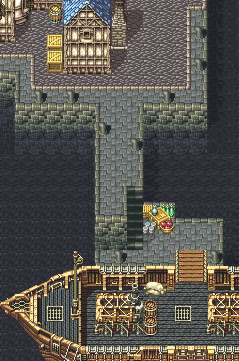
\includegraphics[width=\columnwidth]{./art/chaosincornelia/port.jpg} \end{center}
%
\ofquote{"You must have cannonballs of steel to challenge me!"\\}{Bikke}\\\\
%
When talking to Dyce or other sailors, the party finds out that the port has often been raided by pirates recently.
Usually, the area is protected by Cornelia's guards, but since the disappearance of the princess, the king has recalled all troops to the castle.
The pirates always attack at night and if the party waits around the port until after dark on any day, they will witness a raid.
As the party knows about their plan, they can try to take defensive measures such as setting up an ambush or traps beforehand.
The attack commences with a large pirate ship docking the port and several pirates storming out to pillage the warehouses and other ships.
The pirates are, once again, Captain Bikke's crew, but this time Bikke himself is present as well.
In the ensuing fight, Bikke stays in the back lines and immediately retreats to his ship once he receives any damage. 
There are also some of his men beside him, again roughly one pirate for each party member.
As Bikke likely runs away from this battle, the party may run into him again in the future.
After successfully scaring off the pirates, the sailors at the port are very thankful to the party and offer them free food accommodation for the night.
%
\vfill
%
\ofmonster{Bikke}{2}{
\includegraphics[width=0.2\columnwidth]{./art/chaosincornelia/pirate2.jpg}}
{
	HP: & \hfill 32 & MP: & \hfill 25\\
	STR: & \hfill 1 & DEF: & \hfill 2 \\
	MAG: & \hfill 1 & RES: & \hfill 2 \\
	AGI: & \hfill 2 & Size: & \hfill M\\
}
{\accf{Scimitar}: 1d DMG}
{	
	\mspell{Thunder}{4}{0r}{Single}{3u}{You deal 2d lightning damage to the target}{\lightning}	
	\mtech{Cheer}{5}{0r}{Single}{3u}{The target gains EnSTR for 1 round.}{\enstr}	
}
%
\vfill
%
Below is map of \accf{Cornelia}, there are also some farms outside the city walls that are not shown.
All important locations are marked with numbers and in the following you can find paragraphs with corresponding numbers that give more details about the locations
The party arrives in Cornelia from the southern gate, where two guards stop them as they do
not recognize the adventurers. 
They advise the party to stay clear of the castle and leave the town after finishing their business. 
Most townspeople are too scared to leave their homes since the princess has disappeared.
%
\begin{center} 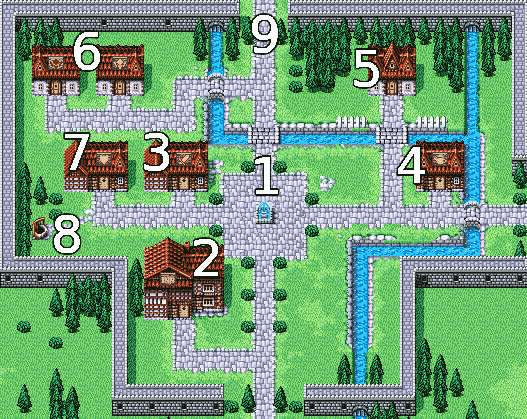
\includegraphics[width=\columnwidth]{./art/chaosincornelia/cornelia.jpg} \end{center}
%
\clearpage
%
\ofquote{"Hello, there! I'm a dancer! What's that? You fancy a dance? Hee hee!"}{Arylon}\\\\
%
\accf{1. Fountain:} The party notices a beautiful fountain standing out in the otherwise unremarkable town.
Nearby is a blue-haired, cheerful, young woman in a red dress who practices dancing, her name is Arylon.
When asked about the princess or the castle, she reveals rumors that princess Sarah is being held hostage for a hefty ransom.
Accordingly, the castle is in chaos and has been locked off.
She also reveals that there have been multiple unsuccessful attempts at rescuing Sarah.
%
\vfill
%
\ofquote{"Please, come in! We charge 50 Gil per night. Would you like to stay?"}{Elia}\\\\
%
\accf{2. Inn:} The party enters into a small room with a red rug on the ground and a counter at its end.
Behind the counter stands a young woman with dark blue hair wearing a long green dress, her name is Elia.
To the left is a large room with multiple beds and minor decorations on the walls where the guests sleep.
To the right is another room, with wooden chairs and tables where guests can sit to eat and drink.
The party can sleep at the Inn for 50 Gil per night per person.  
They can also ask Elia for information, as she overhears a lot from visitors.
She points the party towards various people in town that may need their help such as the smith and the mages.
%
\vfill
%
\accf{3. Smith:} The party enters a large shop with a forge.
Behind the counter is an older man with brown hair and a full beard, his name is Todo.
He informs the party that the store is closed, he cannot work due to not receiving essential shipments from the port.
To help him, the party has to talk to Dyce at Cornelia Port, who is looking after the shipments. 
They consist of a large wooden box on a small wagon, which slightly slows down the carrier's movement.
On their way back to Cornelia, a bizarre monster named \accf{PuPu} makes an attempt to steal the shipments!
PuPu is sitting in the trees, and uses his \accf{Abduct} ability to make the box disappear. 
If the players look for him in the trees while he is doing this, he is easy to spot, because the top of his head is glowing.
Afterwards, he is difficult to spot, a player has to succeed on a check that can vary between DC 6-8.
The party may fail to find PuPu, but he will be nearby if they return later.
If detected, PuPu does not fight, he instead uses \accf{Potions~Please!} and returns the stolen goods if the party complies.
They can also just attack him, in which case the shipment reappears after PuPu is defeated.
Upon successfully returning the cargo, Todo rewards the party with 500 Gil.
The smith can work again, but he will be busy completing outstanding orders for some time.
When the party returns in a few days, Todo may upgrade their weapons or armor and he may sell any Level 1 weapon or armor of your choice.
%
\newpage
%
\ofmonster{PuPu}{?}{
\includegraphics[width=0.15\columnwidth]{./art/chaosincornelia/pupu.jpg}}
{
	HP: & \hfill 10 & MP: & \hfill 10\\
	STR: & \hfill 0 & DEF: & \hfill 0 \\
	MAG: & \hfill 0 & RES: & \hfill 0 \\
	AGI: & \hfill 2 & Size: & \hfill S\\
}
{\accf{Drops}: All abducted objects{}}
{	
	\mtech{Abduct}{0}{1r}{Single}{5u}{
		An object that you can see within range disappears to an unknown location.  
	}{}	
	\mpassive{Potion Please!}{
		Ask your enemies to give you a Potion, if they comply make a DC 8 check.
		If you succeed you disappear to an unknown location (KO), otherwise you keep asking for more Potions.
	}
}
%
\vfill
%
\accf{4. Store:} This general goods store is dominated by a large counter in the center and heaps of wares and items around it.
Behind the counter is a young man with dark hair and a green bandana, his name is Guston.
He is not particularly concerned about the princess, but he is annoyed that the troubles in Cornelia have dampened his sales.
Accordingly, he is very friendly towards potential customers and sells the items listed below.
%
\ofpar
%
\oftable
{p{0.14\columnwidth} p{0.14\columnwidth} l} 
{\accf{Item} & \accf{Price} & \accf{Effect}}
{	
	Echo Grass 		& 50 Gil & Removes Silence.  \ofrow
	Potion 			& 100 Gil & Regain 8 HP. \ofrow
	Ether 			& 150 Gil & The target regains 12 MP. \ofrow
	Phoenix Down	& 300 Gil & Remove KO status and regain 1 HP. \ofrow
	Tent 			& 500 Gil & Allows the party to sleep outside. \ofrow
	Lantern 		& 100 Gil & Illuminates area up to 10u.
}
%
\vfill
%
\ofquote{"Do not lose heart, brave warriors."\\}{Gregory}\\\\
%
\accf{5. Chapel:} The chapel is small and cozy with few wooden banks, but it is also completely empty except for one person, father Gregory.
Gregory is an old man with a long white beard wearing a red hooded robe, he speaks slowly and quietly.
He laments that nobody has been visiting the chapel since the disappearance of Sarah.
Apparently, most townspeople believe that the incident is a divine punishment, so they avoid the chapel.
Gregory asks the party to restore the faith of Cornelia's citizen.
The party can for example convince people by clarifying details about Sarah's disappearance (she was kidnapped), that many are unaware of.
If the party manages to convince at least any 3 people in Cornelia to attend the chapel, Gregory is satisfied and rewards them with 500~Gil.
Moreover, he offers his services to the party for free: he can cure the KO status by performing a 1 hour long ritual.
%
\clearpage
%
\accf{6. The Mages:} These two buildings are almost identical, each one consists of a single large room with a bed and shelves with heaps of magic and alchemy goods and books.
They are inhabited by the eccentric and stubborn twin brothers Gilles and Noah. 
Gilles is a Black Mage who wears a blue robe and a pointed hat, while Noah is a White Mage who wears a white hooded robe with red accents.
The other townspeople usually avoid the brothers, except when they need their services.
Getting annoyed by this, the mages have decided to develop a flask, which allows them to store their magic, so that others can use it without their presence.
Unfortunately, something went wrong during its development, causing the item to break apart in a violent explosion, the result of which the party can see in the back yard.
Out of pride, both of them blame their brother for the accident and they have stopped talking since.
The party can resolve the dispute by convincing them that they were both at fault.
First they have to repair the broken flask either through mechanical or magical means, which is easy.
Then, they have to study the flask and the recipe for creating it, which they can receive from the mages.
A character that can use magic himself immediately understands the issue, one that cannot use magic has to pass a DC 8 check:
the flask broke, because after its creation each mage cast 2 spells into it, causing the flask overload as it cannot hold more than 3 spells.
This can be demonstrated by casting only 3 spells into the flask, which works fine.
If the party manages to convince the mages, they accept their wrongdoing and apologize to each other.
They gift the flask to the party as a token of gratitude and the party may visit them in the future to buy the accessories shown below, to which you may add any other of your choice.
%
\ofpar
%
\oftable
{p{0.28\columnwidth} p{0.15\columnwidth} p{0.47\columnwidth}} 
{\accf{Accessory} & \accf{Price} & \accf{Effect}}
{	
	Magic Flask & 900 Gil & Can store up to 3 spells that are cast into it. The wearer can use an action to unleash a stored spell's effect on a chosen target. \ofrow
	Rune Bracers & 500 Gil & RES +1 \ofrow
	Mythril Shield & 500 Gil & DEF +1
}
%
\vfill
%
\accf{7. Abandoned Building:} This building has been left purposefully empty in case you may need it.
It could be related to one of the character's stories or it may have content that you want to add to the adventure.
Otherwise, the house is empty and the players can ask around to find out that it used to be a shop that has been abandoned due to not being profitable.
%
\vfill
%
\accf{8. Well:} It's a well. It looks like you could climb down it, but you can't. Really.
%
\newpage
%
\accf{9. Castle Entrance:}  This entrance directly leads to \accf{Castle Cornelia} and is permanently blocked by guards.
However, they let the adventurers through if they explain that they want to help find the princess.
The guards ask the party to report to the chancellor on the upper floor.
A map of the castle's ground floor with all relevant location is shown on the right.
The central stairway leads to the throne room, while the back entrance leads to the palace garden.
The palace is filled with armed guards at all times.
%
\ofpar
%
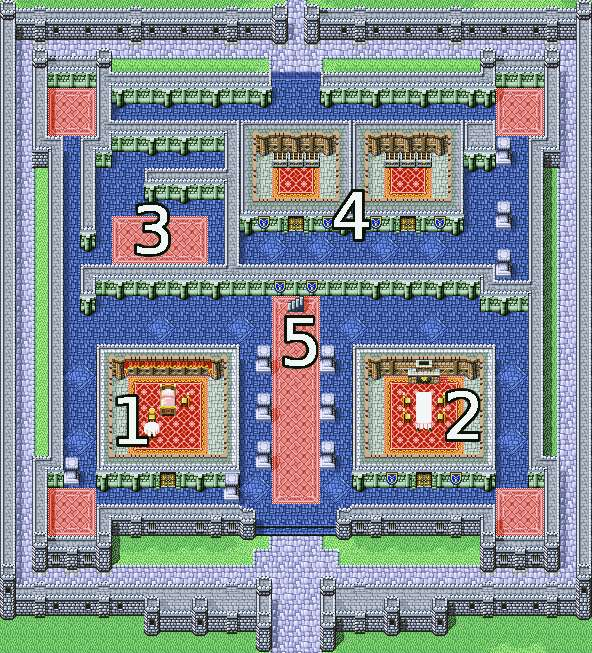
\includegraphics[width=\columnwidth]{./art/chaosincornelia/castle.jpg}
%
\\\\
%
\ofquote{"Please bring my daughter, my Sarah, back to me safely."}{Queen Jayne}\\\\
%
\accf{1. Queen's Room:} Queen Jayne is a middle-aged women with turquoise hair and blue eyes, wearing a long red dress and a golden tiara.
She has been depressed since her daughter's kidnapping and only talks to the party after they have won the king's trust.
Once she talks, she tells the party about the night of the kidnapping, which she has witnessed personally.
On that night, she woke up and encountered Garland who was escaping with the unconscious princess in his arms.
Garland told her to hand over control Cornelia if she wants to see her daughter alive again.
Then he disappeared with Sarah through the back entrance of the palace.
The Queen is traumatized by this event and she blames herself for not preventing it.
%
\ofpar
%
\accf{2. Sisters's Room:} This room is inhabited by Sarah's sister Alison, an emotional teenager who resembles her mother.
The guards at her door tell the party that she has locked herself in and won't open the door.
If they can convince her, for example by assuring that they will save Sarah, she opens the door to talk.
Alison knows her sister well, as she looks up to her very much.
She tells the party about Sarah's passion for music and that her precious lute has disappeared with her.
If the party manages to calm her down, they have a better chance at convincing the king, who is worried about his daughter.
%
\ofpar
%
\ofquote{"Garland was once the greatest knight in the kingdom. But power corrupted him, and he turned away from his own true nature."}{Ian}\\\\
%
\accf{3. Captain:} The captain of the guard is a young man with long blond hair named Ian, he is wearing a decorated heavy armor and a longsword on his back.
He is reluctant to talk the adventurers and they notice that he is missing his left arm. 
If the party has convinced the king, the captain is willing to talk to them about the mission to rescue Sarah, which he led.
Right after Sarah disappeared, him and his men followed Garland and confronted him at the Big Bridge, north of Cornelia.
However, Garland bested all of them in the ensuing battle and the captain was the only one survivor, albeit without his arm.
He is ashamed of his failure and seems deeply disturbed and scared of Garland's power.
%
\ofpar
%
\accf{4. Treasure Room:}
Both rooms of the treasury are guarded by two men in heavy armor.
If the party has obtained a letter from the king, they are given the following items by guards: 
A large Tent that fits the entire party plus a Potion and 200 Gil per party member.
%
\ofpar
%
\ofquote{"Garland is no longer the man I once knew. I beg of you. Please return my daughter to me quickly!"\\}{King of Cornelia}\\\\
%
\accf{5. Throne Room:} The door is guarded by two guards with glaives and heavy armor.
Inside, the king sits on his throne and the chancellor stands beside him.
The king is a middle-aged man with light blue eyes and brown hair with a long brown beard, he is wearing a golden crown and long red robes.
The chancellor is slightly younger with dark hair, also wearing noble clothing.
The king is happy to see the adventurers, as he is desperate to find his daughter, but the chancellor is very skeptical.
In the following conversation, the party can try to convince the king that they can rescue Sarah, but the chancellor convinces him that they have to prove their trustworthiness first.
The king then laments that he has been neglecting his people while trying to rescue his daughter.
He asks the party to help the people of Cornelia to prove that they are capable of saving Sarah, in return he promises to provide them with supplies for the journey.
Completing some of the following tasks may convince the king: help the smith to receive his shipments, resolve the dispute between the two mages, defend the port against the pirates, help the chapel regain its members.
After the party wins the king's trust, he reveals further details on the kidnapping:
Sarah was kidnapped by a former knight of Cornelia named Garland, the most powerful swordsman in the kingdom.
Garland used to be close to the king, but power has corrupted him and he demanded to become his successor. 
When the king denied, Garland abducted his daughter as ransom for control over Cornelia.
Many other knights have tried to save her and even though none succeeded, they found out that Garland keeps Sarah in the Chaos Shrine, north of Cornelia and past the Big Bridge.
The king keeps his promise and writes a letter to confirm that they were officially given the task of rescuing the princess.
This letter allows the party to retrieve supplies from the treasury and other members of the palace are more willing to talk to them.
After successfully convincing the king, the party is also rewarded with a \accf{Level Up}!
%
\ofpar
%
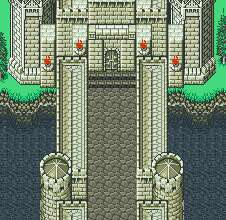
\includegraphics[width=\columnwidth]{./art/chaosincornelia/bridge.jpg} 
%
\\\\
%
\ofquote{"Let's see how you handle the mighty me! And by me, I mean Gilgamesh!! And by handle, I mean DIE!"}{Gilgamesh}\\\\
%
When departing from Cornelia and heading north, the party finds themselves in the forests and grasslands surrounding the city.
After several hours of travel through the quiet nature, they arrive at the Big Bride, which is massive but also old and brittle.
When they reach its end, they encounter Gilgamesh who seems to have been awaiting them.
Gilgamesh is not necessarily good or evil, he travels the world to find powerful weapons for his collection.
Garland has convinced Gilgamesh to work for him, in return he has gifted him the legendary sword "Excalibur".
Upon meeting the party, Gilgamesh recognizes them as potentially worthy opponents and draws his weapons, his combat details are shown below.
When reduced to 0 HP, Gilgamesh does not immediately faint, instead he finally draws Excalibur for one last attack.
Upon trying to use it, the sword deals no damage and immediately breaks.
Gilgamesh realizes that he was tricked and seeing no other option, he flees. 
As he remains alive, the party may meet Gilgamesh again in the future.
The party can now finally cross the bridge to reach the dark forest before the Chaos Shrine.
The forest is unusually quiet and most of its trees and plants seem to have died out.
The adventurers can very likely not reach the Shrine before sunset, so they should rest the night in the forest.\\\\
%
\ofmonster{Gilgamesh}{2}{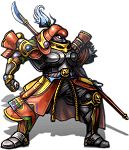
\includegraphics[width=0.2\columnwidth]{./art/chaosincornelia/gilgamesh.jpg}}
{
	HP: & \hfill 45 & MP: & \hfill 40\\
	STR: & \hfill 2 & DEF: & \hfill 1 \\
	MAG: & \hfill 0 & RES: & \hfill 0 \\
	AGI: & \hfill 4 & Size: & \hfill M\\
}
{\accf{Polearm}: 1d DMG \hfill \accf{Drops}: 500 Gil}
{	
	\mtech{Death Claw}{6}{0r}{Single}{Weapon}{
		Make two Attacks against the target and if at least one of them hits, he suffers Immobile for 1 round.
	}{\immobile}	
	\mtech{Sword Dance}{8}{1r}{3u}{Self}{You make an Attack against every enemy in the target area.}{}
	\mreaction{Critical Strength}{When reduced below 20 HP, you gain EnSTR until the end of battle.}	
}
%
\ofpar
%
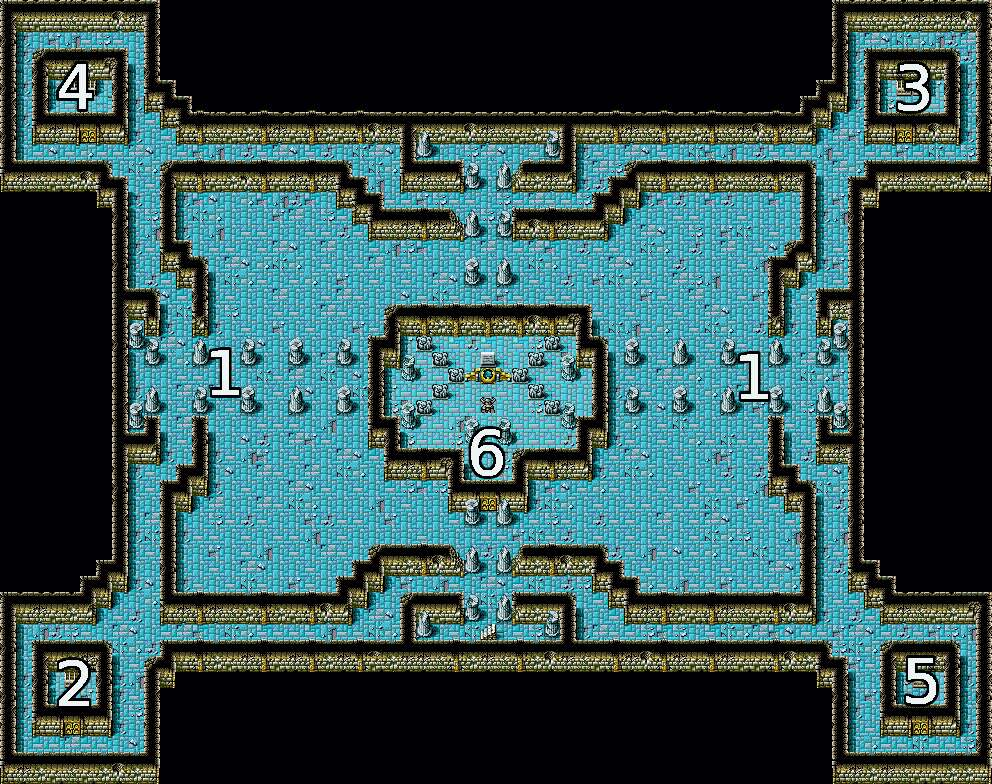
\includegraphics[width=\columnwidth]{./art/chaosincornelia/shrine.jpg} 
%
\\\\
%
As the party reaches the edge of the dark forest, they can see the menacing \accf{Chaos Shrine} in the distance.
As they move closer, they notice that the shine has been claimed by nature, as its walls are damaged and overgrown and the foundation has begun to sink into the ground.
An unnatural serenity surrounds the shrine with no other living being in sight and the only entrance is a set of brittle stairs that lead down into darkness. 
After descending the stairs, the party arrives at the south of the map shown below and can barely see in the dark.
The way north is blocked from rubble that is a product of pillars and large rocks which have broken off from the ceiling.
Upon closer inspection, the party realizes that this blockade has been created purposefully.
%
\newpage
%
\accf{1. Traps:} Both marked locations contain a magical trap on the ground that has been placed by Garland to alert him and  impede intruders.
A character that is actively looking for traps or taking similar precautions notices it by passing a DC~7 check. 
The trap explodes when stepped, dealing 1d+3 fire damage to everyone within 1u of its center. 
%
\ofpar
%
\accf{2. Mimic:} Inside this room is a single large chest that once touched reveals itself to be a vicious Mimic.
A character can notice that something is wrong with the chest beforehand by passing a DC~9 check.
If they fail to do so, the Mimic gets an surprise round at the start of the ensuing battle.
%
\\\\
%
\ofmonster{Mimic}{2}{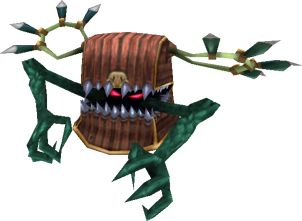
\includegraphics[width=0.28\columnwidth]{./art/chaosincornelia/mimic.jpg}}
{
	HP: & \hfill 20 & MP: & \hfill 0\\
	STR: & \hfill 2 & DEF: & \hfill 0 \\
	MAG: & \hfill 0 & RES: & \hfill 0 \\
	AGI: & \hfill 2 & Size: & \hfill M\\
}
{\accf{Bite}: 1d DMG \hfill \accf{Drops:} 200 Gil}
{}
%
\ofpar
%
\accf{3. Healing Spring:} The heavy door of this room is locked and can be broken or lockpicked, by passing a check whose DC can vary from 6 to 9 depending on the character's expertise.
Inside the room, the party finds a large chalice that stands on a stone pedestal and is filled with what seems to be water.
Upon closer inspection, a character can understand that the liquid is of magical nature and a character that drinks it, fully recovers his HP and MP immediately.
However, the chalice itself has no magical properties and contains only 5 portions of the healing water.
%
\ofpar
%
\accf{4. Chests:} This room contains 2 chests, one can be opened easily and contains 3 Potions and a Phoenix Down.
The other one contains \accf{Sarah's Lute} and can only be lockpicked by passing a check where the DC varies between 7 and 10 depending on the character's expertise.
It can also be opened with a key that Garland carries with himself, but the chest is too robust to be broken through force.
%
\ofpar
%
\accf{5. Secret Door:} This room is empty except for a large stone tablet on the left wall with multiple different symbols on it.
Upon closer inspection, the party can understand that the symbols describe a short music piece. 
The wall next to it contains a secret door which is revealed by playing the piece on Sarah's Lute, which only Sarah herself should able to perform properly enough.
The secret door leads into a small room with a stone pedestal which has a golden ring on it.
The accessory is named \accf{Angel Ring}, it is worth 2000 Gil and has the following effect: when you suffer KO while wearing it, you can activate it to immediately get revived with 1 HP. The ring is destroyed after using this effect.
%
\clearpage
%
\ofquote{"Hmph. The king's lapdogs. Do you have any idea who you're messing with?"}{Garland}\\\\
%
\accf{6. Garland:} At the center of the temple, the party finally confronts Garland.
Sarah is also in this room, locked in a cage that stands in the corner. 
Garland is a tall, well-built man in full heavy armor wearing a purple cape and carrying a sword.
He is very arrogant and believes that he deserves to rule Cornelia, because he is the strongest warrior in the kingdom.
Garland has studied the dark secrets of the Chaos Shrine since his arrival to expand his power.
He sees the party as just another annoyance standing in the way of his grand plans.
%
\vfill
%
\ofquote{”You really think you have what it takes to cross swords with ME? Very well...”}{Garland}\\\\
%
Garland draws his weapon to commence the fight and he also summons multiple bats to aid him, one for each party member.
During the battle, he focuses on his positioning to pick off lone party members while he avoids getting outnumbered himself.
In the original story, Garland uses a magical artifact to escape after being defeated and goes on to become the main antagonist of the game.
If you want to continue the adventure differently, he may also die at hand of the adventurers or you can let the players decide his fate.
After being freed from her prison, Sarah is understandably still very scared and traumatized.
She thanks the party for rescuing her and asks them to find her precious lute, which Garland has taken.
The party can refuse her request to quickly return to Cornelia, which Sarah will understand but not be happy about.
%
\vfill
%
\ofmonster
{Garland}{3}{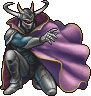
\includegraphics[width=0.2\columnwidth]{./art/chaosincornelia/garland.jpg}}
{
	HP: & \hfill 42 & MP: & \hfill 50\\
	STR: & \hfill 3 & DEF: & \hfill 2 \\
	MAG: & \hfill 2 & RES: & \hfill 1 \\
	AGI: & \hfill 2 & Size: & \hfill M\\
}
{\accf{Longsword}: 1d DMG \hfill \accf{Drops}: 1000 Gil, Key \\ \accf{Auto-Blink, Dual Attack, Revert}}
{
	\mspell{Fire}{4}{0r}{Single}{3u}{The target suffers 2d fire damage.}{}	
	\mspell{Drain}{6}{0r}{Single}{4u}{Reduce the target's HP by 1d and increase yours by the same amount.}{}	
	\mspell{Silence}{6}{0r}{Single}{5u}{The target makes a DC 8 check and suffers Silence for 3 rounds upon failure.}{\silence}
%	\mreaction{Parry}{Whenever you fail to evade an Attack, you can make a DC~8 and when you succeed, the damage you suffer is halved.}
}
%
\newpage
%
\ofmonster
{Bat}{1}{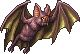
\includegraphics[width=0.2\columnwidth]{./art/chaosincornelia/bat.jpg}}
{
	HP: & \hfill 6 & MP: & \hfill 0\\
	STR: & \hfill 0 & DEF: & \hfill 0 \\
	MAG: & \hfill 0 & RES: & \hfill 2 \\
	AGI: & \hfill 4 & Size: & \hfill S\\
}
{\accf{Teeth}: 1d DMG \hfill \accf{Drops:} 100 Gil }
{\mpassive{Absorb}{On every successful Attack you regain 1d HP.}}
%
\vfill
%
\ofquote{"You... you've come to rescue me? I don't know how I can ever thank you..."}{Sarah}\\\\
%
After rescuing Sarah, the party has to return her safely to Cornelia and therefore, they have to travel back the long way they came from.
The journey should be uneventful, but you can feel free add some surprises of your own.
Sarah is a young princess with turquoise hair like her mother and wears a gold colored dress as well as a golden pendant with red jewels.
She is polite but also very quiet and absent, because she is suffering from the physical and mental scars of the kidnapping.
Sarah is not capable of looking after herself, she needs the adventurers' guidance during the journey.
While travelling, she often asks about the state of Cornelia and her family because she blames herself for what has happened.
%
\vfill
%
\ofquote{"Thank you for returning my daughter to my side."\\}{King of Cornelia}\\\\
%
When entering Cornelia with the princess at their side, the adventurers are hailed as heroes by the townspeople and guards.
The inhabitants of the castle are surprised when meeting the party, as they had already given up on ever seeing the princess again.
The king is very grateful to the adventurers and orders his servants to prepare a banquet in their honor.
Furthermore, the king offers them very generous rewards for rescuing his daughter as he had promised.
In the original story, the king commands his men to rebuild a broken bridge, that leads to another  continent for the adventurers to explore.
Depending on how you want to continue the game, his gift should be something that helps the party on their upcoming adventures.
He could for example gift them a ship that allows them to reach new lands or a house in Cornelia if the city will stay relevant.
By rescuing princess Sarah and defeating Garland, the party has grown together and developed their individual skills.
Accordingly they are rewarded with another \accf{Level Up}!
Even though they still have a lot to learn, they have proven themselves to be capable adventurers that can stand up against the evil in the world.
From here, you can continue the adventure by building on the presented content and creating your own locations, characters and challenges.
%
\clearpage